\documentclass[tikz,border=20pt]{standalone}
\usepackage{tikz}
\usetikzlibrary{shapes,arrows,positioning,decorations.pathreplacing,backgrounds,fit,calc,shadows}
\usepackage{xcolor}

% Define colors
\definecolor{request}{RGB}{33, 150, 243}
\definecolor{security}{RGB}{220, 53, 69}
\definecolor{controller}{RGB}{40, 167, 69}
\definecolor{service}{RGB}{255, 152, 0}
\definecolor{repository}{RGB}{156, 39, 176}
\definecolor{database}{RGB}{16, 142, 233}
\definecolor{cache}{RGB}{255, 193, 7}
\definecolor{audit}{RGB}{108, 117, 125}
\definecolor{external}{RGB}{111, 66, 193}

\begin{document}
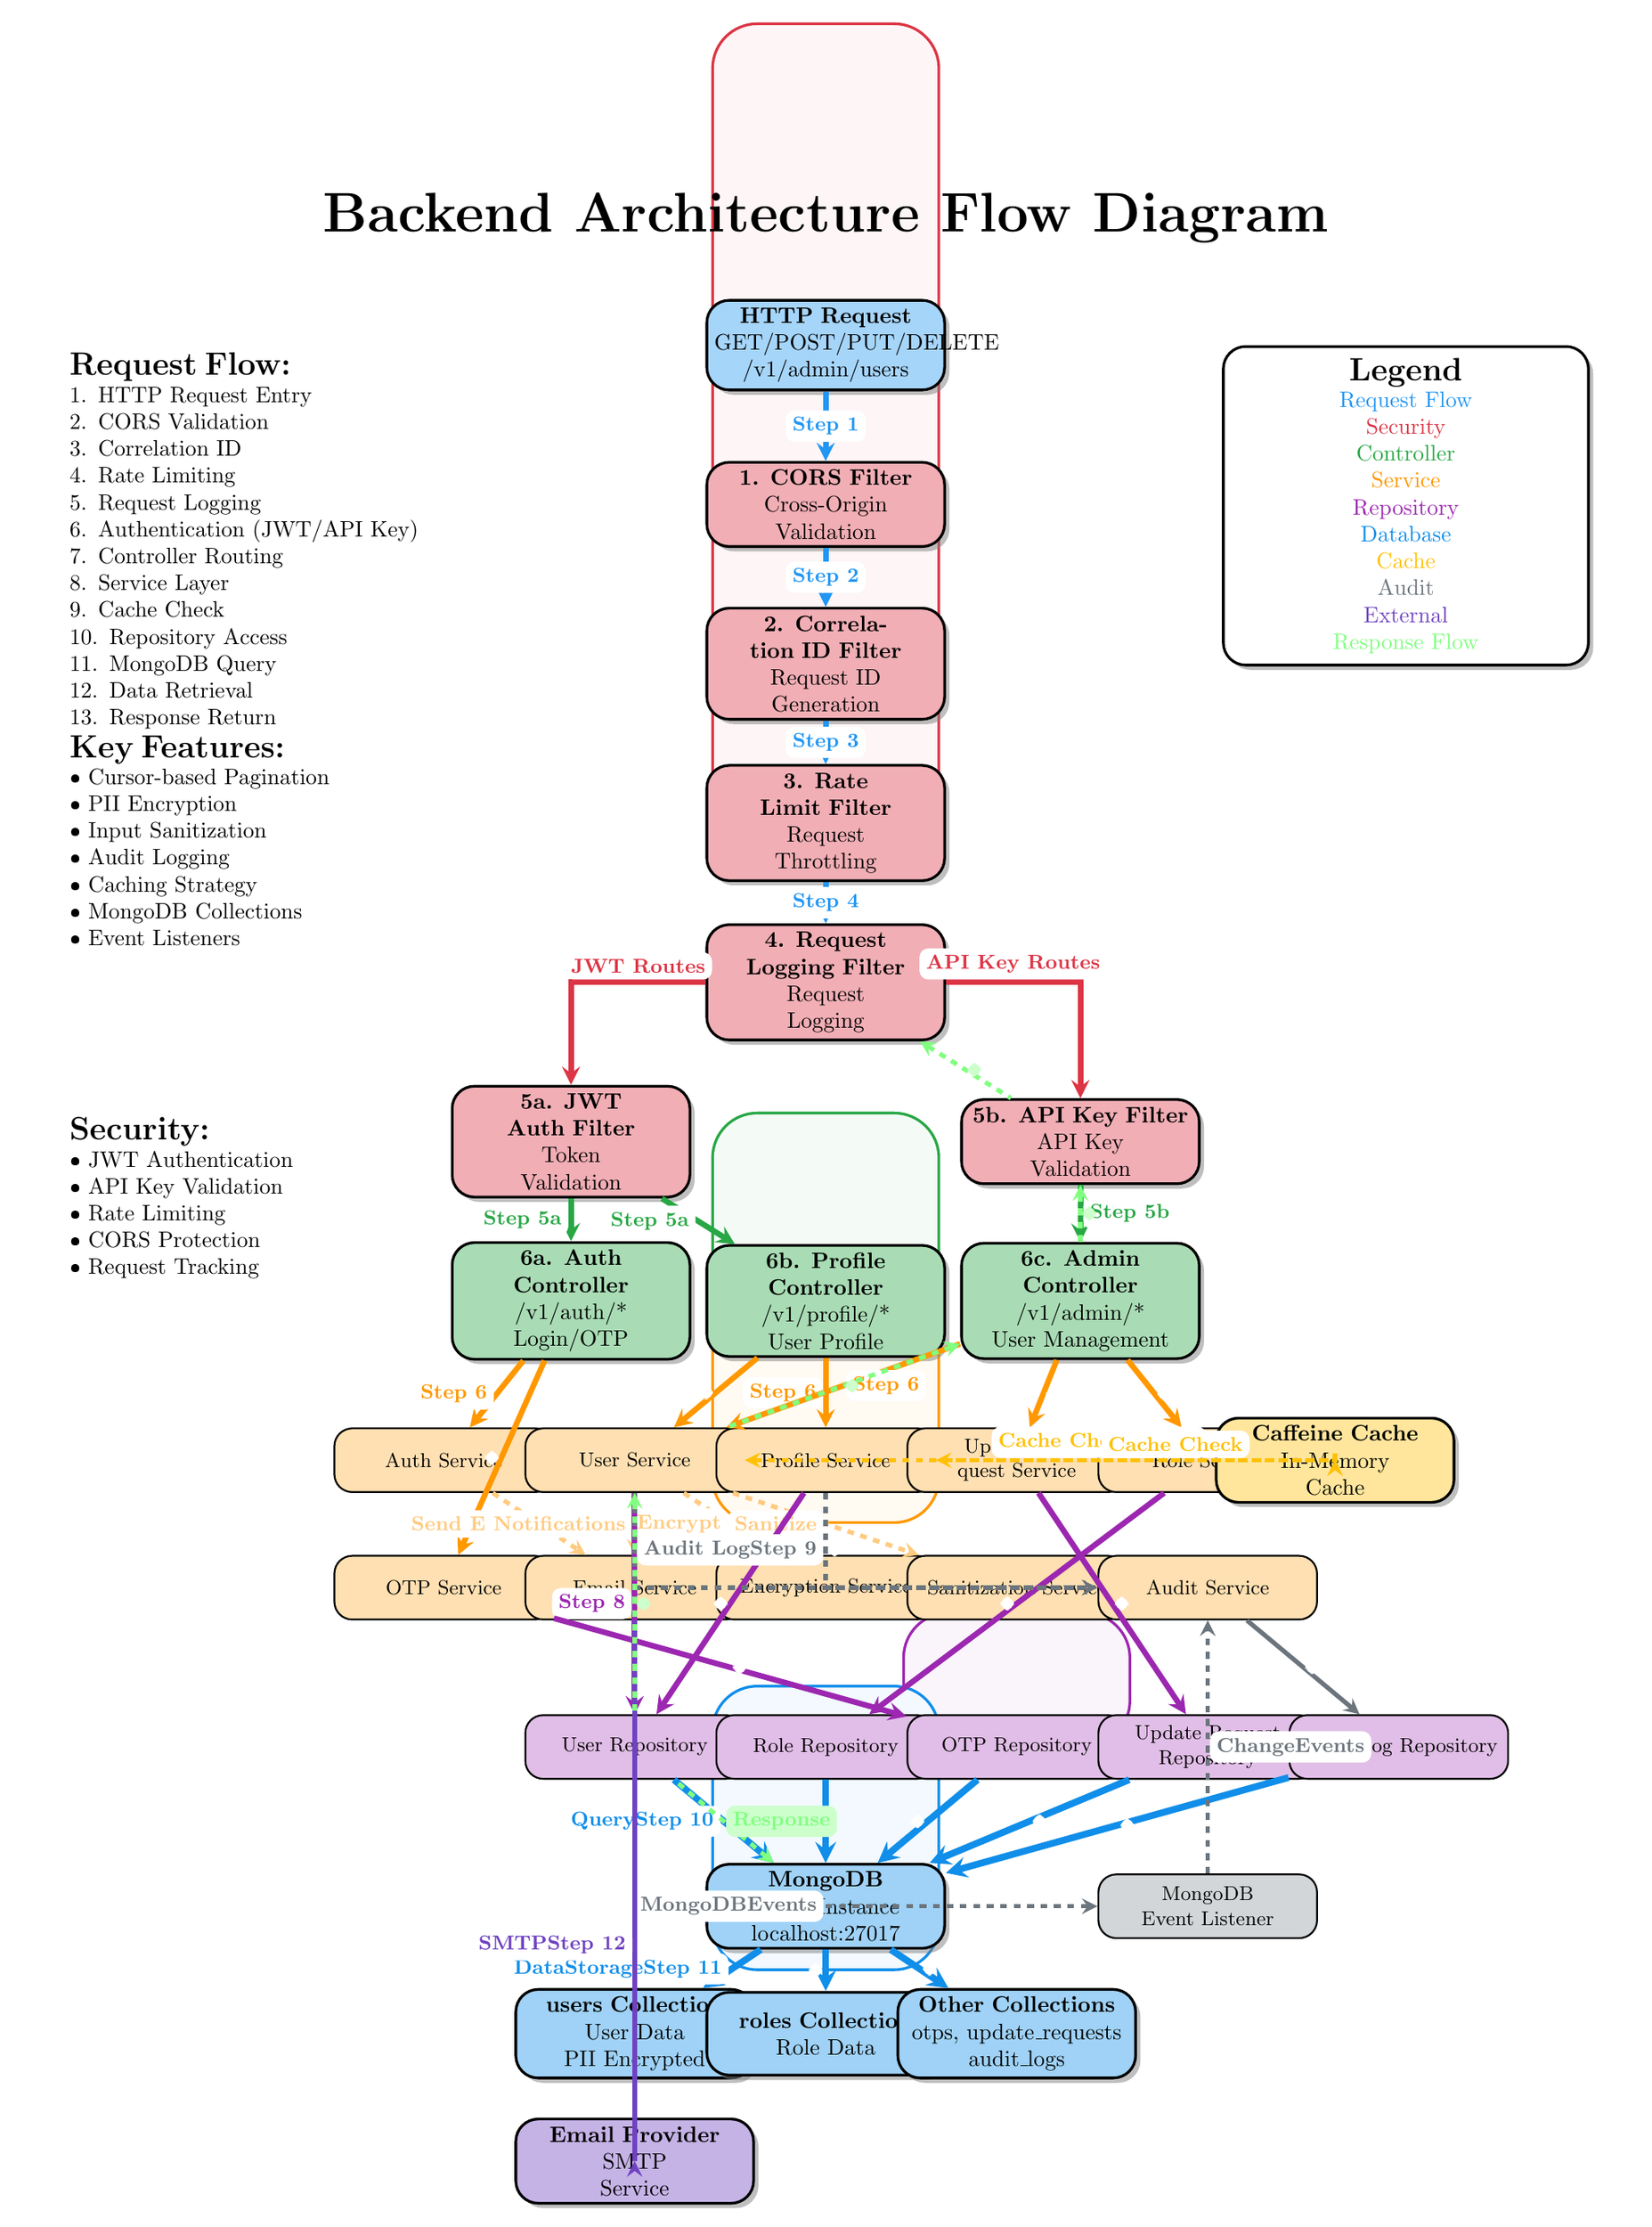
\begin{tikzpicture}[
    node distance=2cm and 3.5cm,
    box/.style={rectangle, rounded corners=10pt, draw=black, very thick, text width=3.5cm, minimum height=1.3cm, text centered, font=\normalsize, drop shadow},
    component/.style={rectangle, rounded corners=8pt, draw=black, thick, text width=3.2cm, minimum height=1cm, text centered, font=\small},
    arrow/.style={->, >=stealth, very thick, line width=2.5pt},
    label/.style={font=\small, above, sloped, text width=2.5cm, align=center},
    flowlabel/.style={font=\small\bfseries, fill=white, rounded corners=4pt, inner sep=3pt}
]

% ========== REQUEST ENTRY POINT ==========
\node[box, fill=request!40] (httpRequest) at (0,14) {\textbf{HTTP Request}\\
    \normalsize GET/POST/PUT/DELETE\\
    \normalsize /v1/admin/users};

% ========== SECURITY FILTERS (SEQUENTIAL) ==========
\node[box, fill=security!40] (corsFilter) at (0,11.5) {\textbf{1. CORS Filter}\\
    \normalsize Cross-Origin\\
    \normalsize Validation};

\node[box, fill=security!40] (correlationFilter) at (0,9) {\textbf{2. Correlation ID Filter}\\
    \normalsize Request ID\\
    \normalsize Generation};

\node[box, fill=security!40] (rateLimitFilter) at (0,6.5) {\textbf{3. Rate Limit Filter}\\
    \normalsize Request\\
    \normalsize Throttling};

\node[box, fill=security!40] (requestLogFilter) at (0,4) {\textbf{4. Request Logging Filter}\\
    \normalsize Request\\
    \normalsize Logging};

\node[box, fill=security!40] (jwtFilter) at (-4,1.5) {\textbf{5a. JWT Auth Filter}\\
    \normalsize Token\\
    \normalsize Validation};

\node[box, fill=security!40] (apiKeyFilter) at (4,1.5) {\textbf{5b. API Key Filter}\\
    \normalsize API Key\\
    \normalsize Validation};

% ========== CONTROLLERS ==========
\node[box, fill=controller!40] (authController) at (-4,-1) {\textbf{6a. Auth Controller}\\
    \normalsize /v1/auth/*\\
    \normalsize Login/OTP};

\node[box, fill=controller!40] (profileController) at (0,-1) {\textbf{6b. Profile Controller}\\
    \normalsize /v1/profile/*\\
    \normalsize User Profile};

\node[box, fill=controller!40] (adminController) at (4,-1) {\textbf{6c. Admin Controller}\\
    \normalsize /v1/admin/*\\
    \normalsize User Management};

% ========== SERVICE LAYER ==========
\node[component, fill=service!30] (authService) at (-6,-3.5) {Auth Service};
\node[component, fill=service!30] (userService) at (-3,-3.5) {User Service};
\node[component, fill=service!30] (profileService) at (0,-3.5) {Profile Service};
\node[component, fill=service!30] (updateService) at (3,-3.5) {Update Request Service};
\node[component, fill=service!30] (roleService) at (6,-3.5) {Role Service};

\node[component, fill=service!30] (otpService) at (-6,-5.5) {OTP Service};
\node[component, fill=service!30] (emailService) at (-3,-5.5) {Email Service};
\node[component, fill=service!30] (encryptionService) at (0,-5.5) {Encryption Service};
\node[component, fill=service!30] (sanitizationService) at (3,-5.5) {Sanitization Service};
\node[component, fill=service!30] (auditService) at (6,-5.5) {Audit Service};

% ========== CACHE ==========
\node[box, fill=cache!40] (cache) at (8,-3.5) {\textbf{Caffeine Cache}\\
    \normalsize In-Memory\\
    \normalsize Cache};

% ========== REPOSITORY LAYER ==========
\node[component, fill=repository!30] (userRepo) at (-3,-8) {User Repository};
\node[component, fill=repository!30] (roleRepo) at (0,-8) {Role Repository};
\node[component, fill=repository!30] (otpRepo) at (3,-8) {OTP Repository};
\node[component, fill=repository!30] (updateRepo) at (6,-8) {Update Request Repository};
\node[component, fill=repository!30] (auditRepo) at (9,-8) {Audit Log Repository};

% ========== DATABASE LAYER ==========
\node[box, fill=database!40] (mongodb) at (0,-10.5) {\textbf{MongoDB}\\
    \normalsize Single Instance\\
    \normalsize localhost:27017};

\node[box, fill=database!40] (usersCollection) at (-3,-12.5) {\textbf{users Collection}\\
    \normalsize User Data\\
    \normalsize PII Encrypted};

\node[box, fill=database!40] (rolesCollection) at (0,-12.5) {\textbf{roles Collection}\\
    \normalsize Role Data};

\node[box, fill=database!40] (otherCollections) at (3,-12.5) {\textbf{Other Collections}\\
    \normalsize otps, update\_requests\\
    \normalsize audit\_logs};

% ========== EXTERNAL SERVICES ==========
\node[box, fill=external!40] (emailProvider) at (-3,-14.5) {\textbf{Email Provider}\\
    \normalsize SMTP\\
    \normalsize Service};

% ========== EVENT LISTENER ==========
\node[component, fill=audit!30] (mongoListener) at (6,-10.5) {MongoDB Event Listener};

% ========== MAIN FLOW ARROWS (SEQUENTIAL) ==========
\draw[arrow, color=request] (httpRequest) -- (corsFilter) node[flowlabel, pos=0.5] {Step 1};
\draw[arrow, color=request] (corsFilter) -- (correlationFilter) node[flowlabel, pos=0.5] {Step 2};
\draw[arrow, color=request] (correlationFilter) -- (rateLimitFilter) node[flowlabel, pos=0.5] {Step 3};
\draw[arrow, color=request] (rateLimitFilter) -- (requestLogFilter) node[flowlabel, pos=0.5] {Step 4};

% ========== AUTHENTICATION BRANCH ==========
\draw[arrow, color=security] (requestLogFilter) -| (jwtFilter) node[flowlabel, pos=0.25, above] {JWT Routes};
\draw[arrow, color=security] (requestLogFilter) -| (apiKeyFilter) node[flowlabel, pos=0.25, above] {API Key Routes};

% ========== CONTROLLER ROUTING ==========
\draw[arrow, color=controller] (jwtFilter) -- (authController) node[flowlabel, pos=0.5, left] {Step 5a};
\draw[arrow, color=controller] (jwtFilter) -- (profileController) node[flowlabel, pos=0.5, left] {Step 5a};
\draw[arrow, color=controller] (apiKeyFilter) -- (adminController) node[flowlabel, pos=0.5, right] {Step 5b};

% ========== CONTROLLER TO SERVICES ==========
\draw[arrow, color=service] (authController) -- (authService) node[flowlabel, pos=0.5, left] {Step 6};
\draw[arrow, color=service] (authController) -- (otpService) node[flowlabel, pos=0.5, left] {};
\draw[arrow, color=service] (profileController) -- (profileService) node[flowlabel, pos=0.5, left] {Step 6};
\draw[arrow, color=service] (profileController) -- (userService) node[flowlabel, pos=0.5, left] {};
\draw[arrow, color=service] (adminController) -- (userService) node[flowlabel, pos=0.5, right] {Step 6};
\draw[arrow, color=service] (adminController) -- (updateService) node[flowlabel, pos=0.5, right] {};
\draw[arrow, color=service] (adminController) -- (roleService) node[flowlabel, pos=0.5, right] {};

% ========== SERVICE DEPENDENCIES ==========
\draw[arrow, color=service!50, dashed, line width=2pt] (userService) -- (encryptionService) node[flowlabel, pos=0.5, left] {PII Encrypt};
\draw[arrow, color=service!50, dashed, line width=2pt] (userService) -- (sanitizationService) node[flowlabel, pos=0.5, left] {Sanitize};
\draw[arrow, color=service!50, dashed, line width=2pt] (authService) -- (emailService) node[flowlabel, pos=0.5, left] {Send Email};
\draw[arrow, color=service!50, dashed, line width=2pt] (userService) -- (emailService) node[flowlabel, pos=0.5, left] {Notifications};

% ========== CACHE OPERATIONS ==========
\draw[arrow, color=cache, dashed, <->, line width=2pt] (userService) -| (cache) node[flowlabel, pos=0.3, above] {Cache Check\\
    Step 7};
\draw[arrow, color=cache, dashed, <->, line width=2pt] (profileService) -| (cache) node[flowlabel, pos=0.3, above] {Cache Check};

% ========== SERVICE TO REPOSITORY ==========
\draw[arrow, color=repository] (userService) -- (userRepo) node[flowlabel, pos=0.5, left] {Step 8};
\draw[arrow, color=repository] (roleService) -- (roleRepo) node[flowlabel, pos=0.5, left] {};
\draw[arrow, color=repository] (otpService) -- (otpRepo) node[flowlabel, pos=0.5, right] {};
\draw[arrow, color=repository] (updateService) -- (updateRepo) node[flowlabel, pos=0.5, right] {};
\draw[arrow, color=repository] (profileService) -- (userRepo) node[flowlabel, pos=0.5, left] {};

% ========== AUDIT FLOW ==========
\draw[arrow, color=audit, dashed, line width=2pt] (userService) |- (auditService) node[flowlabel, pos=0.3, right] {Audit Log\\
    Step 9};
\draw[arrow, color=audit, dashed, line width=2pt] (profileService) |- (auditService) node[flowlabel, pos=0.3, right] {};
\draw[arrow, color=audit, line width=2pt] (auditService) -- (auditRepo) node[flowlabel, pos=0.5, right] {};

% ========== REPOSITORY TO DATABASE ==========
\draw[arrow, color=database, very thick, line width=3pt] (userRepo) -- (mongodb) node[flowlabel, pos=0.5, left] {Query\\
    Step 10};
\draw[arrow, color=database, very thick, line width=3pt] (roleRepo) -- (mongodb) node[flowlabel, pos=0.5, left] {};
\draw[arrow, color=database, very thick, line width=3pt] (otpRepo) -- (mongodb) node[flowlabel, pos=0.5, left] {};
\draw[arrow, color=database, very thick, line width=3pt] (updateRepo) -- (mongodb) node[flowlabel, pos=0.5, right] {};
\draw[arrow, color=database, very thick, line width=3pt] (auditRepo) -- (mongodb) node[flowlabel, pos=0.5, right] {};

% ========== MONGODB TO COLLECTIONS ==========
\draw[arrow, color=database, very thick, line width=3pt] (mongodb) -- (usersCollection) node[flowlabel, pos=0.5, left] {Data\\
    Storage\\
    Step 11};
\draw[arrow, color=database, very thick, line width=3pt] (mongodb) -- (rolesCollection) node[flowlabel, pos=0.5, left] {};
\draw[arrow, color=database, very thick, line width=3pt] (mongodb) -- (otherCollections) node[flowlabel, pos=0.5, right] {};

% ========== EVENT LISTENER ==========
\draw[arrow, color=audit, dashed, line width=2pt] (mongodb) |- (mongoListener) node[flowlabel, pos=0.3, left] {MongoDB\\
    Events};
\draw[arrow, color=audit, dashed, line width=2pt] (mongoListener) -- (auditService) node[flowlabel, pos=0.5, right] {Change\\
    Events};

% ========== EMAIL PROVIDER ==========
\draw[arrow, color=external, line width=2pt] (emailService) |- (emailProvider) node[flowlabel, pos=0.3, left] {SMTP\\
    Step 12};

% ========== RESPONSE FLOW (REVERSE) ==========
\draw[arrow, color=green!50, dashed, <-, line width=2pt] (mongodb) -- (userRepo) node[flowlabel, pos=0.5, right, fill=green!20] {Response};
\draw[arrow, color=green!50, dashed, <-, line width=2pt] (userService) -- (userRepo) node[flowlabel, pos=0.5, right, fill=green!20] {};
\draw[arrow, color=green!50, dashed, <-, line width=2pt] (adminController) -- (userService) node[flowlabel, pos=0.5, right, fill=green!20] {};
\draw[arrow, color=green!50, dashed, <-, line width=2pt] (apiKeyFilter) -- (adminController) node[flowlabel, pos=0.5, right, fill=green!20] {};
\draw[arrow, color=green!50, dashed, <-, line width=2pt] (requestLogFilter) -- (apiKeyFilter) node[flowlabel, pos=0.5, right, fill=green!20] {};

% ========== BACKGROUND LAYERS ==========
\begin{scope}[on background layer]
    \node[fit=(corsFilter)(correlationFilter)(rateLimitFilter)(requestLogFilter)(jwtFilter)(apiKeyFilter), 
          fill=security!5, draw=security, very thick, rounded corners=20pt, inner sep=15pt, 
          label={[font=\large\bfseries, anchor=south west, yshift=-8pt]south west:Security Layer (Filters)}] {};
    
    \node[fit=(authController)(profileController)(adminController), 
          fill=controller!5, draw=controller, very thick, rounded corners=20pt, inner sep=15pt,
          label={[font=\large\bfseries, anchor=south west, yshift=-8pt]south west:Controller Layer}] {};
    
    \node[fit=(authService)(userService)(profileService)(updateService)(roleService)(otpService)(emailService)(encryptionService)(sanitizationService)(auditService), 
          fill=service!5, draw=service, very thick, rounded corners=20pt, inner sep=15pt,
          label={[font=\large\bfseries, anchor=south west, yshift=-8pt]south west:Service Layer}] {};
    
    \node[fit=(userRepo)(roleRepo)(otpRepo)(updateRepo)(auditRepo), 
          fill=repository!5, draw=repository, very thick, rounded corners=20pt, inner sep=15pt,
          label={[font=\large\bfseries, anchor=south west, yshift=-8pt]south west:Repository Layer}] {};
    
    \node[fit=(mongodb)(usersCollection)(rolesCollection)(otherCollections), 
          fill=database!5, draw=database, very thick, rounded corners=20pt, inner sep=15pt,
          label={[font=\large\bfseries, anchor=south west, yshift=-8pt]south west:Database Layer (MongoDB)}] {};
\end{scope}

% ========== TITLE ==========
\node[font=\Huge\bfseries, text width=25cm, align=center] (title) at (0,16) {Backend Architecture Flow Diagram};

% ========== FLOW DESCRIPTION ==========
\node[font=\normalsize, text width=6cm, align=left, anchor=north west] (flowDesc) at (-12,14) {\textbf{\Large Request Flow:}\\
    \normalsize 1. HTTP Request Entry\\
    \normalsize 2. CORS Validation\\
    \normalsize 3. Correlation ID\\
    \normalsize 4. Rate Limiting\\
    \normalsize 5. Request Logging\\
    \normalsize 6. Authentication (JWT/API Key)\\
    \normalsize 7. Controller Routing\\
    \normalsize 8. Service Layer\\
    \normalsize 9. Cache Check\\
    \normalsize 10. Repository Access\\
    \normalsize 11. MongoDB Query\\
    \normalsize 12. Data Retrieval\\
    \normalsize 13. Response Return};

\node[font=\normalsize, text width=6cm, align=left, anchor=north west] (features) at (-12,8) {\textbf{\Large Key Features:}\\
    \normalsize • Cursor-based Pagination\\
    \normalsize • PII Encryption\\
    \normalsize • Input Sanitization\\
    \normalsize • Audit Logging\\
    \normalsize • Caching Strategy\\
    \normalsize • MongoDB Collections\\
    \normalsize • Event Listeners};

\node[font=\normalsize, text width=6cm, align=left, anchor=north west] (security) at (-12,2) {\textbf{\Large Security:}\\
    \normalsize • JWT Authentication\\
    \normalsize • API Key Validation\\
    \normalsize • Rate Limiting\\
    \normalsize • CORS Protection\\
    \normalsize • Request Tracking};

% ========== LEGEND ==========
\node[box, fill=white, text width=5.5cm, minimum height=5cm, anchor=north east] (legend) at (12,14) {\textbf{\Large Legend}\\
    \normalsize \textcolor{request}{Request Flow}\\
    \normalsize \textcolor{security}{Security}\\
    \normalsize \textcolor{controller}{Controller}\\
    \normalsize \textcolor{service}{Service}\\
    \normalsize \textcolor{repository}{Repository}\\
    \normalsize \textcolor{database}{Database}\\
    \normalsize \textcolor{cache}{Cache}\\
    \normalsize \textcolor{audit}{Audit}\\
    \normalsize \textcolor{external}{External}\\
    \normalsize \textcolor{green!50}{Response Flow}};

\end{tikzpicture}
\end{document}
